\chapter{Rozszerzenia modelu licencjonowania}\label{chap:extensions}

\section{Przegląd badanych wariantów}

Oprócz bazowych konfiguracji \texttt{duolingo\_super} i \texttt{roman\_domination} rozważono osiem rozszerzeń licencyjnych. Warianty \texttt{duolingo\_p\_2}, \texttt{duolingo\_p\_4} oraz \texttt{duolingo\_p\_5} odzwierciedlają rodzinne plany o stałej opłacie grupowej obejmującej odpowiednio $2$, $4$ i $5$ osób. Z kolei \texttt{roman\_p\_3}, \texttt{roman\_p\_4} i \texttt{roman\_p\_5} modyfikują koszt licencji grupowej w modelu dominowania (stała pojemność, koszt $p \in \{3,4,5\}$). Dwa ostatnie warianty odnoszą się do rzeczywistych ofert: \texttt{spotify} dodaje plan Duo (pojemność 2) pomiędzy licencją indywidualną a rodzinną, natomiast \texttt{netflix} umożliwia korzystanie z planów dla 1, 2 lub 4 osób. Podstawowe statystyki dla wszystkich konfiguracji zestawiono w tab.~\ref{tab:ext-overall-static}. W każdym przypadku ponownie analizowano ten sam zestaw algorytmów, pomijając obserwacje z \texttt{timeout}.

\begin{table}[H]
  \centering
  \caption{Statystyki agregowane dla rozszerzeń (benchmark statyczny).}
  \label{tab:ext-overall-static}
  \begin{tabular}{lrrrrr}
    \toprule
    \textbf{Konfiguracja} & \textbf{Med. koszt} & \textbf{Med. koszt/węzeł} & \textbf{Śr. koszt/węzeł} & \textbf{Med. czas [s]} & \textbf{Śr. czas [s]} \\
    \midrule
    duolingo\_p\_2        & 40.00               & 0.500                     & 0.554                    & 0.157                  & 0.637                 \\
    duolingo\_p\_4        & 66.50               & 0.820                     & 0.860                    & 0.181                  & 0.677                 \\
    duolingo\_p\_5        & 81.00               & 0.920                     & 0.982                    & 0.162                  & 0.938                 \\
    spotify               & 32.97               & 0.408                     & 0.479                    & 0.120                  & 0.547                 \\
    netflix               & 58.06               & 0.662                     & 0.729                    & 0.105                  & 0.623                 \\
    roman\_p\_3           & 44.00               & 0.547                     & 0.585                    & 0.127                  & 0.477                 \\
    roman\_p\_4           & 51.00               & 0.660                     & 0.701                    & 0.128                  & 0.475                 \\
    roman\_p\_5           & 56.00               & 0.750                     & 0.800                    & 0.114                  & 0.493                 \\
  \end{tabular}
\end{table}

\section{Warianty rodziny Duolingo}

Zmiana limitu liczby osób obejmowanych jedną opłatą dramatycznie wpływa na koszt. W tab.~\ref{tab:ext-duolingo-static} widać, że przy planie obejmującym dwie osoby (\texttt{duolingo\_p\_2}) metaheurystyki redukują koszt na węzeł o 14\% względem zachłannego rozwiązania, zachowując czasy na poziomie ułamka sekundy (algorytm genetyczny) lub 1--1,2~s (mrówki, tabu). Podwyższenie limitu do czterech lub pięciu osób istotnie zwiększa koszt na węzeł -- wartości dla metaheurystyk rosną odpowiednio do $0{,}78$ oraz $0{,}91$ -- co dobrze ilustruje rys.~\ref{fig:ext-duolingo-cost}. Równocześnie czasy wykonania pozostają niewrażliwe na rozmiar planu (rys.~\ref{fig:ext-duolingo-time}), ponieważ różnica wynika głównie z ceny, a nie z trudności rebalansowania.

\begin{table}[H]
  \centering
  \caption{Mediany (koszt/węzeł, czas) dla kluczowych algorytmów -- rodzina Duolingo.}
  \label{tab:ext-duolingo-static}
  \begin{tabular}{llrr}
    \toprule
    \textbf{Konfiguracja} & \textbf{Algorytm}   & \textbf{Med. koszt/węzeł} & \textbf{Med. czas [s]} \\
    \midrule
    duolingo\_p\_2        & Algorytm zachłanny  & 0.515                     & 0.000                  \\
    duolingo\_p\_2        & Algorytm genetyczny & 0.460                     & 0.364                  \\
    duolingo\_p\_2        & Algorytm mrówkowy   & 0.440                     & 1.146                  \\
    duolingo\_p\_2        & Przeszukiwanie tabu & 0.465                     & 1.184                  \\
    duolingo\_p\_4        & Algorytm zachłanny  & 0.843                     & 0.000                  \\
    duolingo\_p\_4        & Algorytm genetyczny & 0.760                     & 0.489                  \\
    duolingo\_p\_4        & Algorytm mrówkowy   & 0.798                     & 1.383                  \\
    duolingo\_p\_4        & Przeszukiwanie tabu & 0.783                     & 0.961                  \\
    duolingo\_p\_5        & Algorytm zachłanny  & 0.937                     & 0.001                  \\
    duolingo\_p\_5        & Algorytm genetyczny & 0.897                     & 0.539                  \\
    duolingo\_p\_5        & Algorytm mrówkowy   & 0.900                     & 1.688                  \\
    duolingo\_p\_5        & Przeszukiwanie tabu & 0.910                     & 0.741                  \\
  \end{tabular}
\end{table}

\begin{figure}[H]
  \centering
  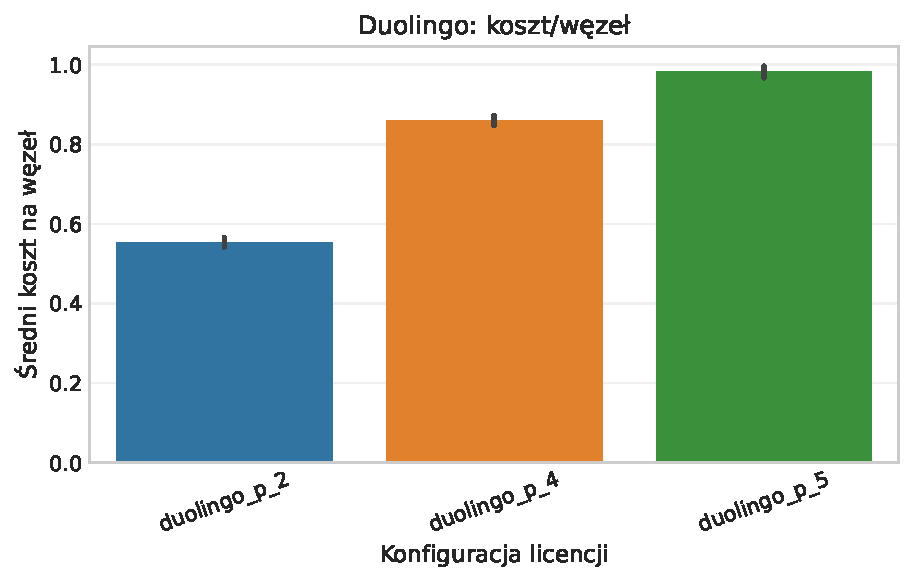
\includegraphics[width=0.6\linewidth]{assets/figures/extensions/static/duolingo_cost_per_node_comparison.pdf}
  \caption{Koszt na węzeł w zależności od planu Duolingo (mediany kluczowych algorytmów).}
  \label{fig:ext-duolingo-cost}
\end{figure}

\begin{figure}[H]
  \centering
  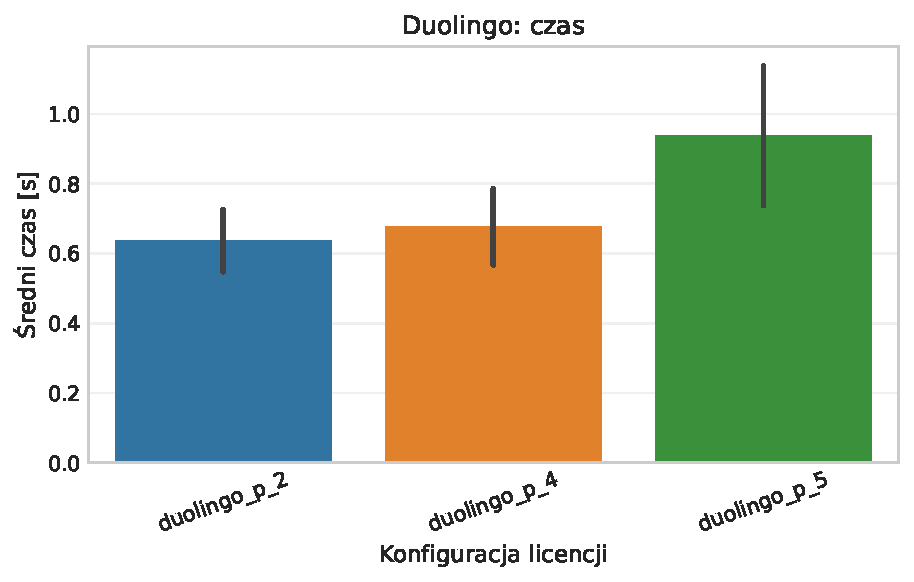
\includegraphics[width=0.6\linewidth]{assets/figures/extensions/static/duolingo_time_comparison.pdf}
  \caption{Czas wykonania dla planów Duolingo (mediany kluczowych algorytmów).}
  \label{fig:ext-duolingo-time}
\end{figure}

Zmiana struktury licencji przekłada się również na udział planów grupowych (tab.~\ref{tab:ext-license-mix}). W planie dwuosobowym ponad połowa przydziałów wykorzystuje licencję grupową, podczas gdy w wariancie pięcioosobowym udział grup spada do 24\% -- algorytmy preferują licencje indywidualne, bo koszt planu grupowego rośnie szybciej niż łączna cena kilku kont Solo.

\section{Warianty dominowania rzymskiego}

Podnoszenie kosztu licencji grupowej w modelu Roman ($p=3\ldots5$) prowadzi do stopniowego spadku przewagi nad rozwiązaniami zachłannymi (tab.~\ref{tab:ext-roman-static}). Dla $p=3$ wciąż obserwujemy redukcję kosztu na węzeł o 7--13\% względem heurystyk, lecz dla $p=5$ metaheurystyki są zaledwie odrobinę lepsze (różnice rzędu –0,005 do –0,04). Wysoki koszt planu grupowego wymusza korzystanie z licencji Solo, co potwierdza rosnący udział bloków indywidualnych w tab.~\ref{tab:ext-license-mix}.

\begin{table}[H]
  \centering
  \caption{Mediany (koszt/węzeł, czas) dla kluczowych algorytmów -- rodzina Roman.}
  \label{tab:ext-roman-static}
  \begin{tabular}{llrr}
    \toprule
    \textbf{Konfiguracja} & \textbf{Algorytm}   & \textbf{Med. koszt/węzeł} & \textbf{Med. czas [s]} \\
    \midrule
    roman\_p\_3           & Algorytm zachłanny  & 0.597                     & 0.000                  \\
    roman\_p\_3           & Algorytm genetyczny & 0.510                     & 0.276                  \\
    roman\_p\_3           & Algorytm mrówkowy   & 0.535                     & 0.656                  \\
    roman\_p\_3           & Przeszukiwanie tabu & 0.545                     & 0.684                  \\
    roman\_p\_4           & Algorytm zachłanny  & 0.695                     & 0.000                  \\
    roman\_p\_4           & Algorytm genetyczny & 0.640                     & 0.358                  \\
    roman\_p\_4           & Algorytm mrówkowy   & 0.665                     & 0.717                  \\
    roman\_p\_4           & Przeszukiwanie tabu & 0.640                     & 0.515                  \\
    roman\_p\_5           & Algorytm zachłanny  & 0.780                     & 0.000                  \\
    roman\_p\_5           & Algorytm genetyczny & 0.750                     & 0.364                  \\
    roman\_p\_5           & Algorytm mrówkowy   & 0.755                     & 0.806                  \\
    roman\_p\_5           & Przeszukiwanie tabu & 0.750                     & 0.330                  \\
  \end{tabular}
\end{table}

\begin{figure}[H]
  \centering
  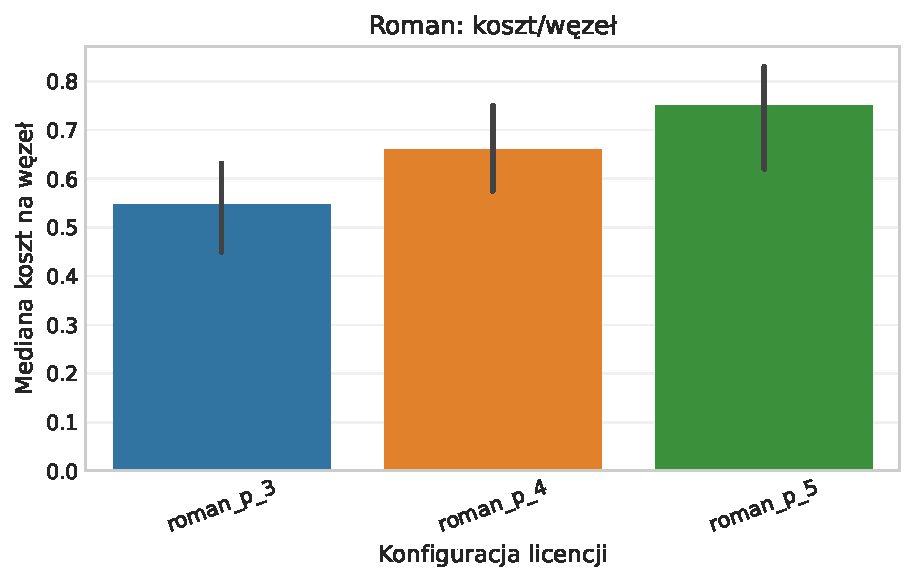
\includegraphics[width=0.6\linewidth]{assets/figures/extensions/static/roman_cost_per_node_comparison.pdf}
  \caption{Koszt na węzeł dla wariantów dominowania rzymskiego.}
  \label{fig:ext-roman-cost}
\end{figure}

\begin{figure}[H]
  \centering
  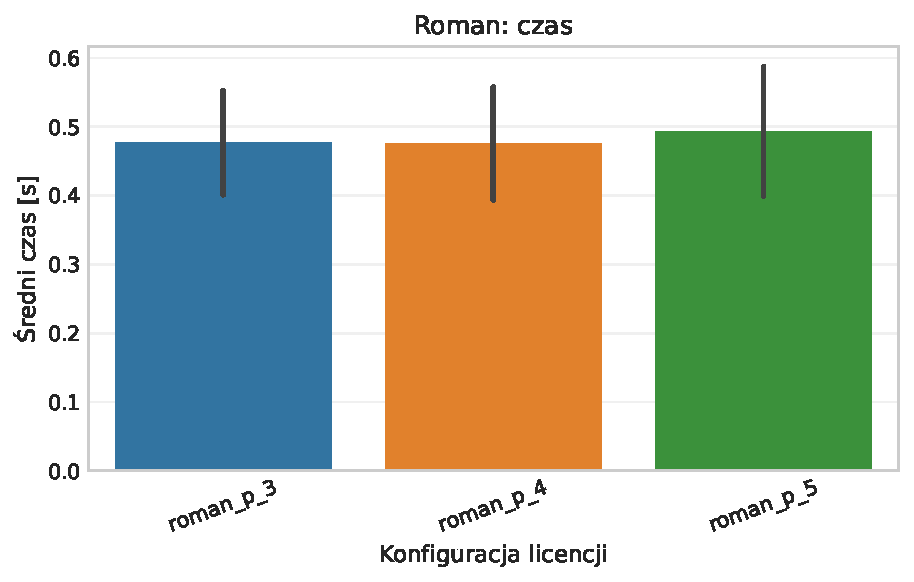
\includegraphics[width=0.6\linewidth]{assets/figures/extensions/static/roman_time_comparison.pdf}
  \caption{Czas wykonania dla wariantów dominowania rzymskiego.}
  \label{fig:ext-roman-time}
\end{figure}

\section{Spotify i Netflix -- dodatkowe plany pośrednie}

Spotify wprowadza trzecią licencję (Duo), co otwiera możliwość parowania użytkowników zamiast budowania dużych grup. Tabela~\ref{tab:ext-additional-static} potwierdza, że przeszukiwanie tabu i algorytm genetyczny osiągają najniższe koszty ($0{,}335$ i $0{,}400$ na węzeł), wyraźnie dystansując heurystykę zachłanną. Rys.~\ref{fig:ext-license-cost} i~\ref{fig:ext-license-time} prezentują pełne porównanie licencji; szczególnie widać, że trzeci plan redukuje koszt bez istotnego wzrostu czasu wykonania. W przypadku Netflixa plan Standard (pojemność 2) wypełnia lukę między kontem solo a planem rodzinnych czterech kont, dzięki czemu metaheurystyki utrzymują koszt w granicach $0{,}60$–$0{,}65$ przy czasie poniżej 1~s.

\begin{table}[H]
  \centering
  \caption{Mediany dla konfiguracji Spotify i Netflix.}
  \label{tab:ext-additional-static}
  \begin{tabular}{llrr}
    \toprule
    \textbf{Konfiguracja} & \textbf{Algorytm}   & \textbf{Med. koszt/węzeł} & \textbf{Med. czas [s]} \\
    \midrule
    spotify               & Algorytm zachłanny  & 0.446                     & 0.000                  \\
    spotify               & Algorytm genetyczny & 0.400                     & 0.229                  \\
    spotify               & Algorytm mrówkowy   & 0.391                     & 1.040                  \\
    spotify               & Przeszukiwanie tabu & 0.335                     & 0.958                  \\
    netflix               & Algorytm zachłanny  & 0.682                     & 0.000                  \\
    netflix               & Algorytm genetyczny & 0.650                     & 0.237                  \\
    netflix               & Algorytm mrówkowy   & 0.656                     & 1.289                  \\
    netflix               & Przeszukiwanie tabu & 0.604                     & 0.999                  \\
  \end{tabular}
\end{table}

\begin{figure}[H]
  \centering
  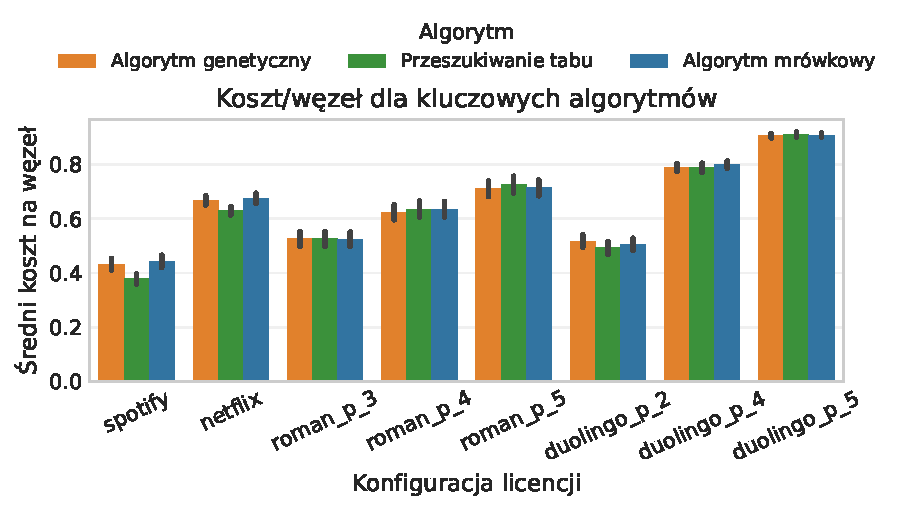
\includegraphics[width=0.6\linewidth]{assets/figures/extensions/static/cost_per_node_by_license_targets.pdf}
  \caption{Koszt na węzeł dla wszystkich rozszerzeń (mediany).}
  \label{fig:ext-license-cost}
\end{figure}

\begin{figure}[H]
  \centering
  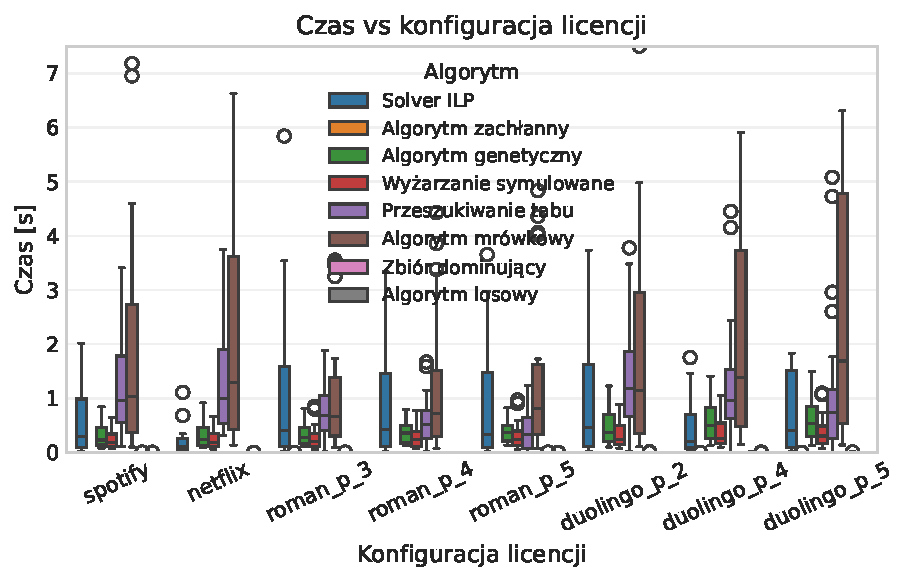
\includegraphics[width=0.6\linewidth]{assets/figures/extensions/static/time_by_license_all_algos.pdf}
  \caption{Czas wykonania dla wszystkich rozszerzeń (mediany).}
  \label{fig:ext-license-time}
\end{figure}

Struktura wykorzystania licencji zmienia się znacząco (tab.~\ref{tab:ext-license-mix}). W Spotify licencje grupowe odpowiadają za 64\% przydziałów (plan Duo + rodzina), podczas gdy w wariancie \texttt{duolingo\_p\_5} udział grup spada do 24\%. W Netflixie większość przydziałów to plany Standard/Premium (udział 68\%).

\begin{table}[H]
  \centering
  \caption{Udział licencji grupowych i indywidualnych (benchmark statyczny).}
  \label{tab:ext-license-mix}
  \begin{tabular}{lrr}
    \toprule
    \textbf{Konfiguracja} & \textbf{Udział grup} & \textbf{Udział indywidualnych} \\
    \midrule
    duolingo\_p\_2        & 0.56                 & 0.44                           \\
    duolingo\_p\_4        & 0.34                 & 0.66                           \\
    duolingo\_p\_5        & 0.24                 & 0.76                           \\
    spotify               & 0.64                 & 0.36                           \\
    netflix               & 0.68                 & 0.32                           \\
    roman\_p\_3           & 0.43                 & 0.57                           \\
    roman\_p\_4           & 0.34                 & 0.66                           \\
    roman\_p\_5           & 0.24                 & 0.76                           \\
  \end{tabular}
\end{table}

\section{Rozszerzenia w środowisku dynamicznym}

Symulacje rebalansowania licencji uwzględniające mutacje sieci (sekcja~\ref{chap:dynamic}) wykonano również dla nowych konfiguracji. Wyniki zagregowane z trzech scenariuszy realistycznych (preferencyjne i triadyczne dołączanie, losowe przełączanie krawędzi) zebrano w tab.~\ref{tab:ext-dyn-overall}. Najniższe koszty osiąga wariant Spotify (mediana $0{,}407$), co wynika z możliwości parowania użytkowników; kolejne w zestawieniu pozostają \texttt{duolingo\_p\_2} oraz \texttt{roman\_p\_3}.

\begin{table}[H]
  \centering
  \caption{Średnie i mediany w symulacjach dynamicznych (ciepły start).}
  \label{tab:ext-dyn-overall}
  \begin{tabular}{lrrrr}
    \toprule
    \textbf{Konfiguracja} & \textbf{Med. koszt/węzeł} & \textbf{Śr. koszt/węzeł} & \textbf{Med. czas [s]} & \textbf{Śr. czas [s]} \\
    \midrule
    duolingo\_p\_2        & 0.488                     & 0.539                    & 0.365                  & 0.939                 \\
    duolingo\_p\_4        & 0.805                     & 0.855                    & 0.355                  & 0.987                 \\
    duolingo\_p\_5        & 0.916                     & 0.980                    & 0.359                  & 0.980                 \\
    spotify               & 0.407                     & 0.467                    & 0.256                  & 0.881                 \\
    netflix               & 0.640                     & 0.714                    & 0.234                  & 0.891                 \\
    roman\_p\_3           & 0.494                     & 0.554                    & 0.287                  & 0.798                 \\
    roman\_p\_4           & 0.600                     & 0.666                    & 0.313                  & 0.930                 \\
    roman\_p\_5           & 0.711                     & 0.763                    & 0.258                  & 0.829                 \\
  \end{tabular}
\end{table}

Różnice względem zimnego startu heurystyki zachłannej przedstawia tab.~\ref{tab:ext-dyn-delta}. Dla większości konfiguracji metaheurystyki redukują koszt na węzeł o 5--12\%, choć okupują to wydłużeniem czasu rebalansowania o 0,4--2,4~s. Wariant \texttt{duolingo\_p\_5} praktycznie traci przewagę kosztową (różnice bliskie zera), natomiast w Spotify przeszukiwanie tabu utrzymuje najwyższą redukcję (–0,087) przy czasie około 1,6~s.

\begin{table}[H]
  \centering
  \caption{Różnice względem algorytmu zachłannego (symulacje dynamiczne, ciepły start).}
  \label{tab:ext-dyn-delta}
  \begin{tabular}{llrr}
    \toprule
    \textbf{Konfiguracja} & \textbf{Algorytm}   & \textbf{$\Delta$ koszt/węzeł} & \textbf{$\Delta$ czas [s]} \\
    \midrule
    duolingo\_p\_2        & Algorytm genetyczny & $-0.059$                      & $+0.647$                   \\
    duolingo\_p\_2        & Algorytm mrówkowy   & $-0.046$                      & $+1.973$                   \\
    duolingo\_p\_2        & Przeszukiwanie tabu & $-0.052$                      & $+2.242$                   \\
    duolingo\_p\_4        & Algorytm genetyczny & $-0.075$                      & $+0.649$                   \\
    duolingo\_p\_4        & Algorytm mrówkowy   & $-0.029$                      & $+2.209$                   \\
    duolingo\_p\_4        & Przeszukiwanie tabu & $-0.043$                      & $+1.558$                   \\
    duolingo\_p\_5        & Algorytm genetyczny & $-0.031$                      & $+0.712$                   \\
    duolingo\_p\_5        & Algorytm mrówkowy   & $+0.001$                      & $+2.480$                   \\
    duolingo\_p\_5        & Przeszukiwanie tabu & $+0.014$                      & $+1.193$                   \\
    spotify               & Algorytm genetyczny & $-0.049$                      & $+0.390$                   \\
    spotify               & Algorytm mrówkowy   & $-0.037$                      & $+1.713$                   \\
    spotify               & Przeszukiwanie tabu & $-0.087$                      & $+1.626$                   \\
    netflix               & Algorytm genetyczny & $-0.075$                      & $+0.403$                   \\
    netflix               & Algorytm mrówkowy   & $-0.031$                      & $+2.200$                   \\
    netflix               & Przeszukiwanie tabu & $-0.087$                      & $+1.656$                   \\
    roman\_p\_3           & Algorytm genetyczny & $-0.039$                      & $+0.448$                   \\
    roman\_p\_3           & Algorytm mrówkowy   & $-0.039$                      & $+1.055$                   \\
    roman\_p\_3           & Przeszukiwanie tabu & $-0.064$                      & $+1.200$                   \\
    roman\_p\_4           & Algorytm genetyczny & $-0.032$                      & $+0.507$                   \\
    roman\_p\_4           & Algorytm mrówkowy   & $-0.023$                      & $+1.200$                   \\
    roman\_p\_4           & Przeszukiwanie tabu & $-0.043$                      & $+1.061$                   \\
    roman\_p\_5           & Algorytm genetyczny & $-0.039$                      & $+0.530$                   \\
    roman\_p\_5           & Algorytm mrówkowy   & $+0.000$                      & $+1.269$                   \\
    roman\_p\_5           & Przeszukiwanie tabu & $-0.005$                      & $+0.363$                   \\
  \end{tabular}
\end{table}

Pełne przebiegi kosztów i czasów dla algorytmów genetycznego oraz mrówkowego w wariantach syntetycznych zebrano na rys.~\ref{fig:dyn-synth-genetic-cost}--\ref{fig:dyn-synth-aco-time}, natomiast ich odpowiedniki dla scenariuszy realistycznych pokazano na rys.~\ref{fig:dyn-real-genetic-cost}--\ref{fig:dyn-real-aco-time}. W każdym przypadku plan Spotify charakteryzuje się najszybszą stabilizacją kosztów, natomiast wariant \texttt{duolingo\_p\_5} wykazuje najwyższy dryf wynikający z większego kosztu licencji grupowej.

\section{Wnioski}

Rozszerzenia licencyjne pozwalają modelować szerokie spektrum ofert rynkowych. Najważniejsze obserwacje to:
\begin{itemize}
  \item Niskie mnożniki planów rodzinnych (\texttt{duolingo\_p\_2}, \texttt{spotify}) znacząco poprawiają koszt na węzeł, a metaheurystyki redukują wynik o 10--20\% względem heurystyk przy niewielkim wzroście czasu.
  \item Wysokie koszty planów grupowych (\texttt{duolingo\_p\_5}, \texttt{roman\_p\_5}) sprawiają, że zysk z metaheurystyk maleje, a dominować zaczynają licencje indywidualne.
  \item W środowisku dynamicznym konfiguracje z planem pośrednim (Spotify, Netflix Standard) utrzymują koszty na najniższym poziomie, a rebalansowanie pozostaje szybkie (do 1~s dla algorytmu genetycznego, ok.~1,6~s dla tabu).
\end{itemize}

Dane potwierdzają, że rozszerzenie modelu o dodatkowe typy licencji umożliwia bardziej elastyczne dopasowanie planów do struktury sieci, a jednocześnie nie zdejmuje z metaheurystyk roli głównego narzędzia optymalizacji kosztów.
